\subsection{Temporal Evidence Accumulation}
\label{subsec:results_temporal}

This experiment empirically evaluates the sequential decision-making dynamics of the \gls{snn} architecture. 
By extracting predictive snapshots at $t=2$ ($20\text{ms}$), $t=5$ ($50\text{ms}$), and $t=10$ ($100\text{ms}$), we can observe the internal state evolution as the network integrates incoming spikes into a stable bounding box regression. 
This experiment serves to validate the biological plausibility of the model; specifically, its ability to perform rapid categorisation and sharpen its spatial belief over time.

\subsubsection*{Qualitative Evidence: Bounding Box Sharpening}

Figure \ref{fig:temporal_sequences} illustrates the predictive evolution for three representative validation samples
across three snapshots at $t=2$ ($20\text{ms}$), $t=5$ ($50\text{ms}$), and $t=10$ ($100\text{ms}$).
\begin{figure}[htbp]
    \centering
    \begin{subfigure}[b]{0.95\textwidth}
        \centering
        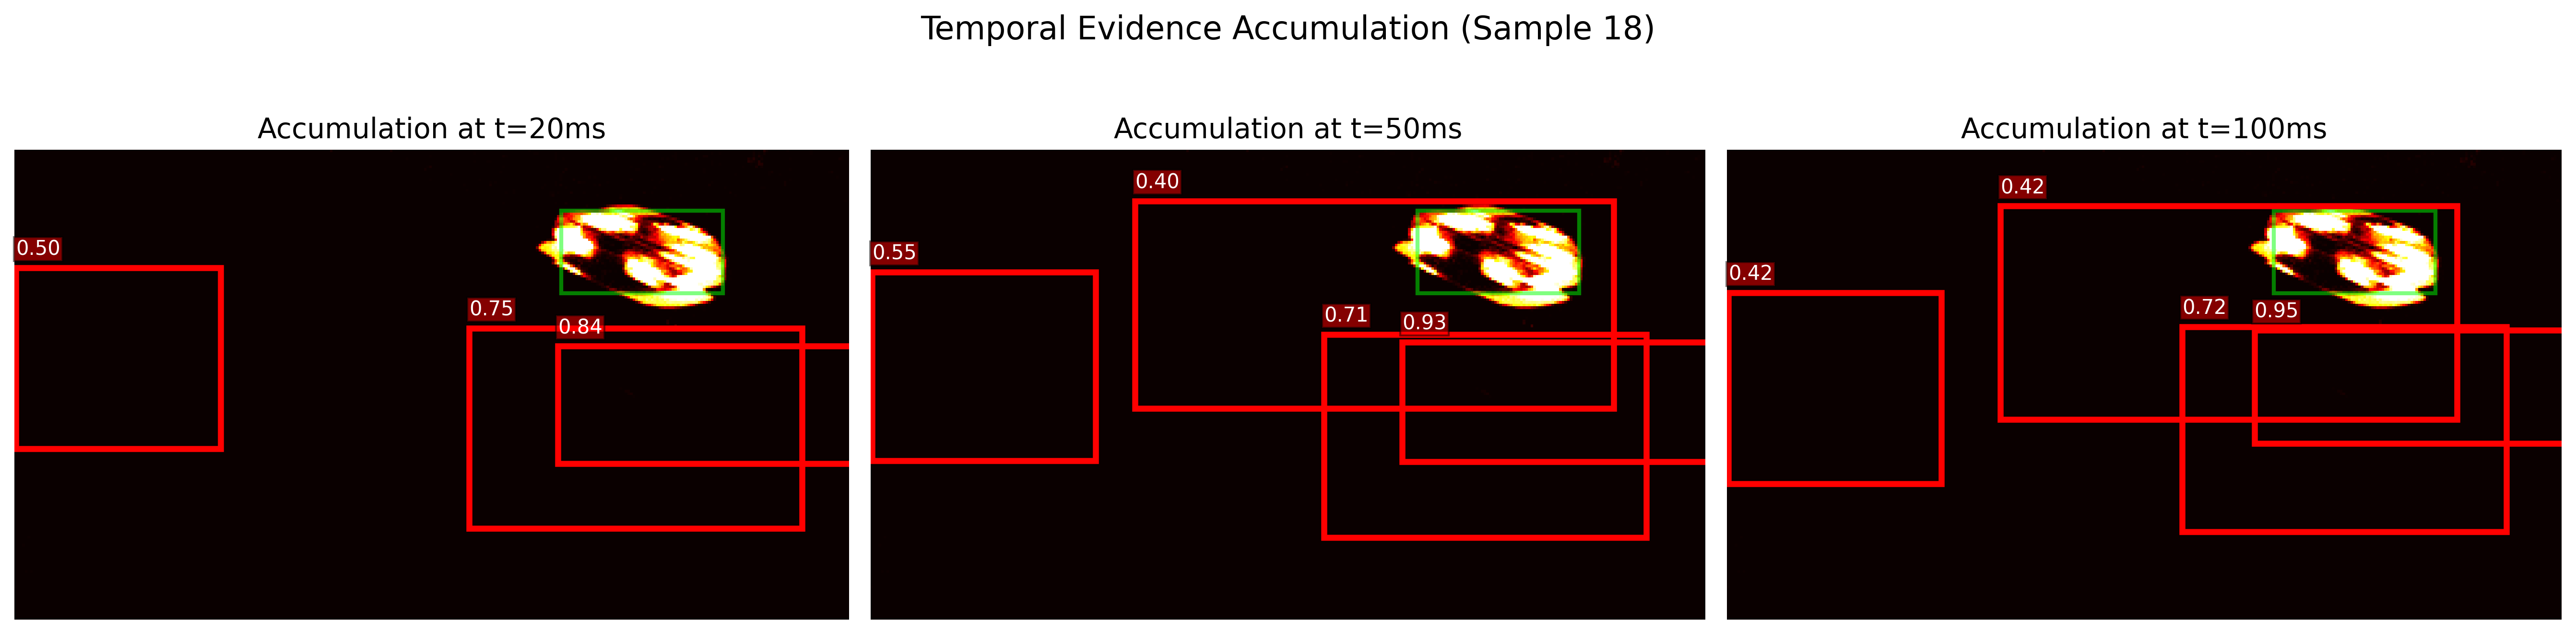
\includegraphics[width=\textwidth]{chapter_3/dnx_results/exp4_temporal/sequence_0.png}
        \caption{Temporal Sequence 1: Initial hunting behaviour and edge consolidation.}
        \label{fig:temp_seq_0}
    \end{subfigure}
    
    \vspace{1.5em}
    
    \begin{subfigure}[b]{0.95\textwidth}
        \centering
        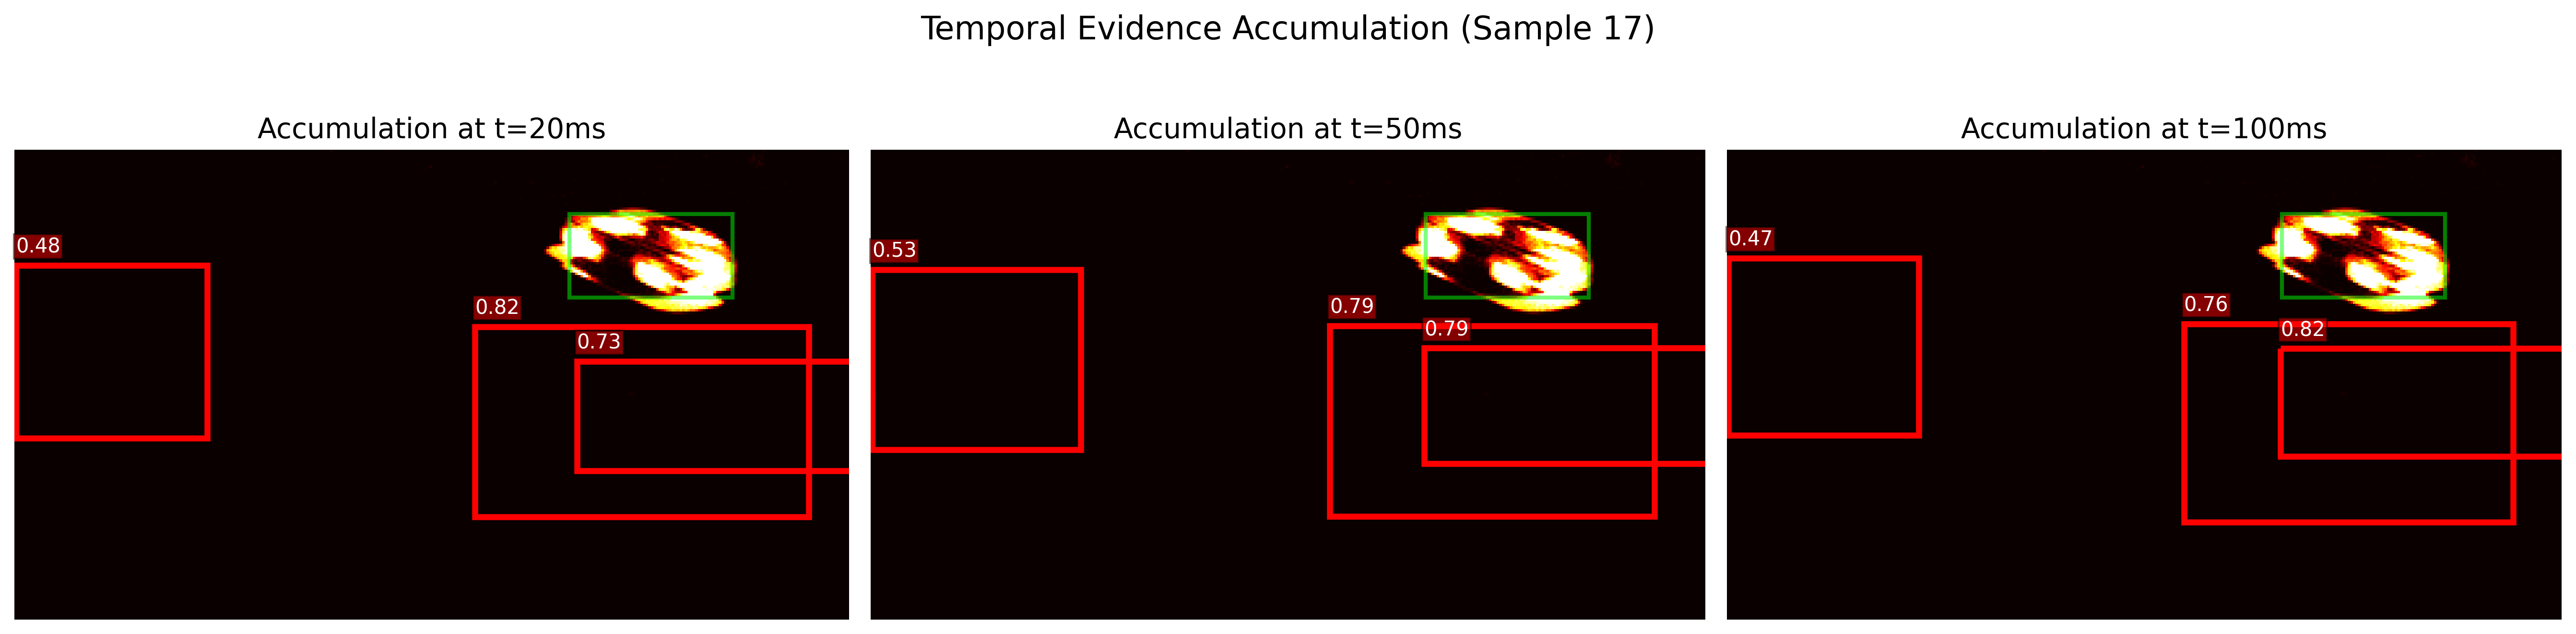
\includegraphics[width=\textwidth]{chapter_3/dnx_results/exp4_temporal/sequence_2.png}
        \caption{Temporal Sequence 2: Persistent hunting with partial sharpening.}
        \label{fig:temp_seq_1}
    \end{subfigure}
    
    \vspace{1.5em}
    
    \begin{subfigure}[b]{0.95\textwidth}
        \centering
        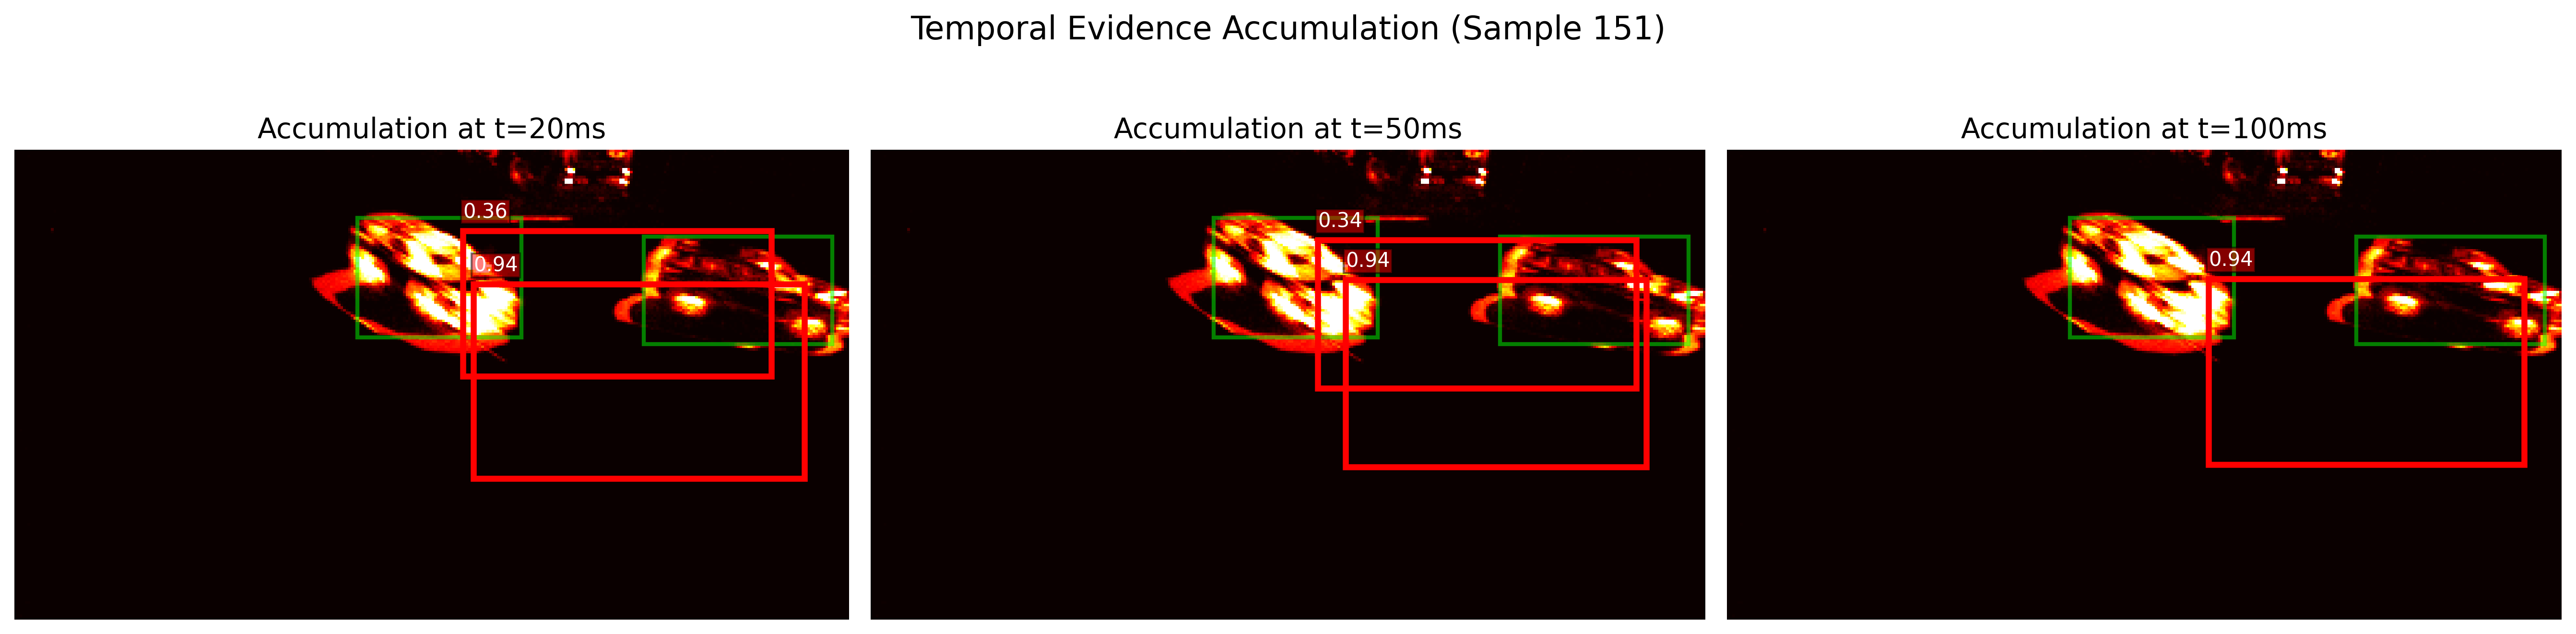
\includegraphics[width=\textwidth]{chapter_3/dnx_results/exp4_temporal/sequence_4.png}
        \caption{Temporal Sequence 3: High-confidence early detection.}
        \label{fig:temp_seq_2}
    \end{subfigure}
    
    \caption[Temporal Evidence Accumulation Sequences]{Evolution of SNN bounding box predictions over $T=10$ timesteps, with annotated confidence scores. Each row demonstrates the progression from sparse initial evidence to a stable, high-confidence detection.}
    \label{fig:temporal_sequences}
\end{figure}

\subsubsection*{Critical Analysis}
As established in the hypothesis (Section \ref{subsec:temporal_evidence}), the early-stage snapshots ($t=2$) exhibit high coordinate jitter and lower confidence, as the \gls{lif} neurons have only begun to aggregate sufficient membrane potential to overcome the firing threshold.
Each sample in Figure \ref{fig:temporal_sequences} exhibits different behaviours:

\paragraph{Hunting Behaviour:}
Figure \ref{fig:temp_seq_2} most clearly demonstrates this phenomenon. At $t=20\text{ms}$, multiple 
overlapping predictions scatter across a dense event cluster with moderate confidences 
($0.43$--$0.56$), indicating early spike activity is sufficient to localise the scene 
region but insufficient to resolve individual vehicle boundaries. At $t=50\text{ms}$, 
a spurious detection emerges with no underlying event support, characteristic of the 
regression head briefly committing to a spatially incorrect region as membrane 
potentials oscillate. By $t=100\text{ms}$, partial consolidation occurs, and the model successfully
observes the car that is partially visible in the top left corner,
yet overlapping boxes and inconsistent confidence scores persist.
This behaviour is consistent with competing spike trains from multiple event sources (i.e. cars) preventing stable threshold-crossing consensus,
meaning that the bounding boxes never truly settle --- hunting without resolution.
It can be attributed to the scene being too spatially complex for the network to disentangle,
highlighting a limitation of this current architecture, and showing an area for future work to increase its complexity to handle such scenes more successfully.

\paragraph{Bounding Box Sharpening:}
Figure \ref{fig:temp_seq_0} best shows this phenomenon: at $t=2$, the initial guess is nowhere near the ground truth, since the majority 
of \gls{lif} neurons have not accumulated sufficient membrane potential to cross the firing threshold ($V_{th} = 0.2$).
However, as time progresses, the model correctly starts to localise on the car, and by $t=10$ settles down into a stable prediction with a confidence of $53\%$.
This sample in particular shows an area for further development, where a post-detection step could be introduced to accumulate nested predictions into one large prediction, which would prevent phenomena such as the one observed here: where there are two nested bounding boxes being drawn for the same event.

\paragraph{High-confidence early detection:}
Figure \ref{fig:temp_seq_2} shows that the current architecture succeeds in high-confidence early detection,
correctly detecting the car in the bottom right corner with a confidence of $91\%$ at the first timestep $t=2$ ($20$\,ms).
In the context of vehicle detection which is time-sensitive, this is a significant finding because it proves that the model can support low-latency prediction accurately.

\todo[inline]{Fix Inconsistencies and rewrite prose.}